\documentclass[varwidth=true]{standalone}
\usepackage{tikz}
\begin{document}
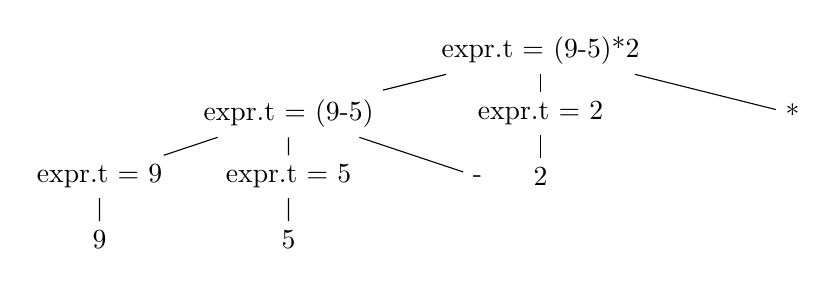
\begin{tikzpicture}[scale=0.8]
  \node (e) at (0, 0) {expr.t = (9-5)*2};

  \node (e95) at (-4, -1) {expr.t = (9-5)};
  \node (e2) at (0, -1) {expr.t = 2};
  \node (*) at (4, -1) {*};
  \draw (e) -- (e95);
  \draw (e) -- (e2);
  \draw (e) -- (*);

  \node (e9) at (-7, -2) {expr.t = 9};
  \node (e5) at (-4, -2) {expr.t = 5};
  \node (-) at (-1, -2) {-};
  \draw (e95) -- (e9);
  \draw (e95) -- (e5);
  \draw (e95) -- (-);

  \node (2) at (0, -2) {2};
  \draw (e2) -- (2);

  \node (9) at (-7, -3) {9};
  \draw (e9) -- (9);

  \node (5) at (-4, -3) {5};
  \draw (e5) -- (5);
\end{tikzpicture}
\end{document}
